% ════════════════════════════════════════════════════════════════════
% SECTION 4 — SYSTEM ARCHITECTURE AND METHODOLOGY
% ════════════════════════════════════════════════════════════════════
\section{System Architecture and Methodology}\label{sec:method}

\subsection{Architecture overview}

\begin{sloppypar}
Figure~\ref{fig:arch} shows the complete system. Six simulated
clients---labelled neutrally A--F (plain identifiers; the labels
carry no geographic or institutional mapping, and no real institution
participates in this study)---each hold a private, non-IID shard of the
benchmark. In every communication round, each selected
client trains a local copy of the shared model on its shard (with an
imbalance-robust loss, described below), and transmits its model
parameters to the aggregation server (the implementation transports
full weight tensors both directions; delta/weight-increment encoding
and quantised uplinks are the communication-cost model's future
compression path, not what the code does). The server forms the next global
model by size-weighted averaging, broadcasts it to all clients, and
the cycle repeats for $T = 50$ rounds. Downstream of federation, the
global model emits flare probabilities; the evaluation of this paper
finds that its calibration and frozen operating points do not survive
the prevalence shift, so no alerting claim is made. Any downstream
use---CME propagation and storm forecasting, geomagnetic-hazard
estimation, GIC and power-system response modelling---would require
components this paper does not evaluate, and the
flare$\to$CME$\to$storm$\to$GIC chain is far from the quantity
modelled here (Section~\ref{sec:limitations}). The division of labour
is deliberate: everything that touches raw magnetogram data (loading,
local training) executes inside the client boundary; everything the
server touches is a weight tensor.
\end{sloppypar}

\begin{figure}[t]
    \centering
    \begin{adjustbox}{max width=\textwidth, max height=0.46\textheight}
        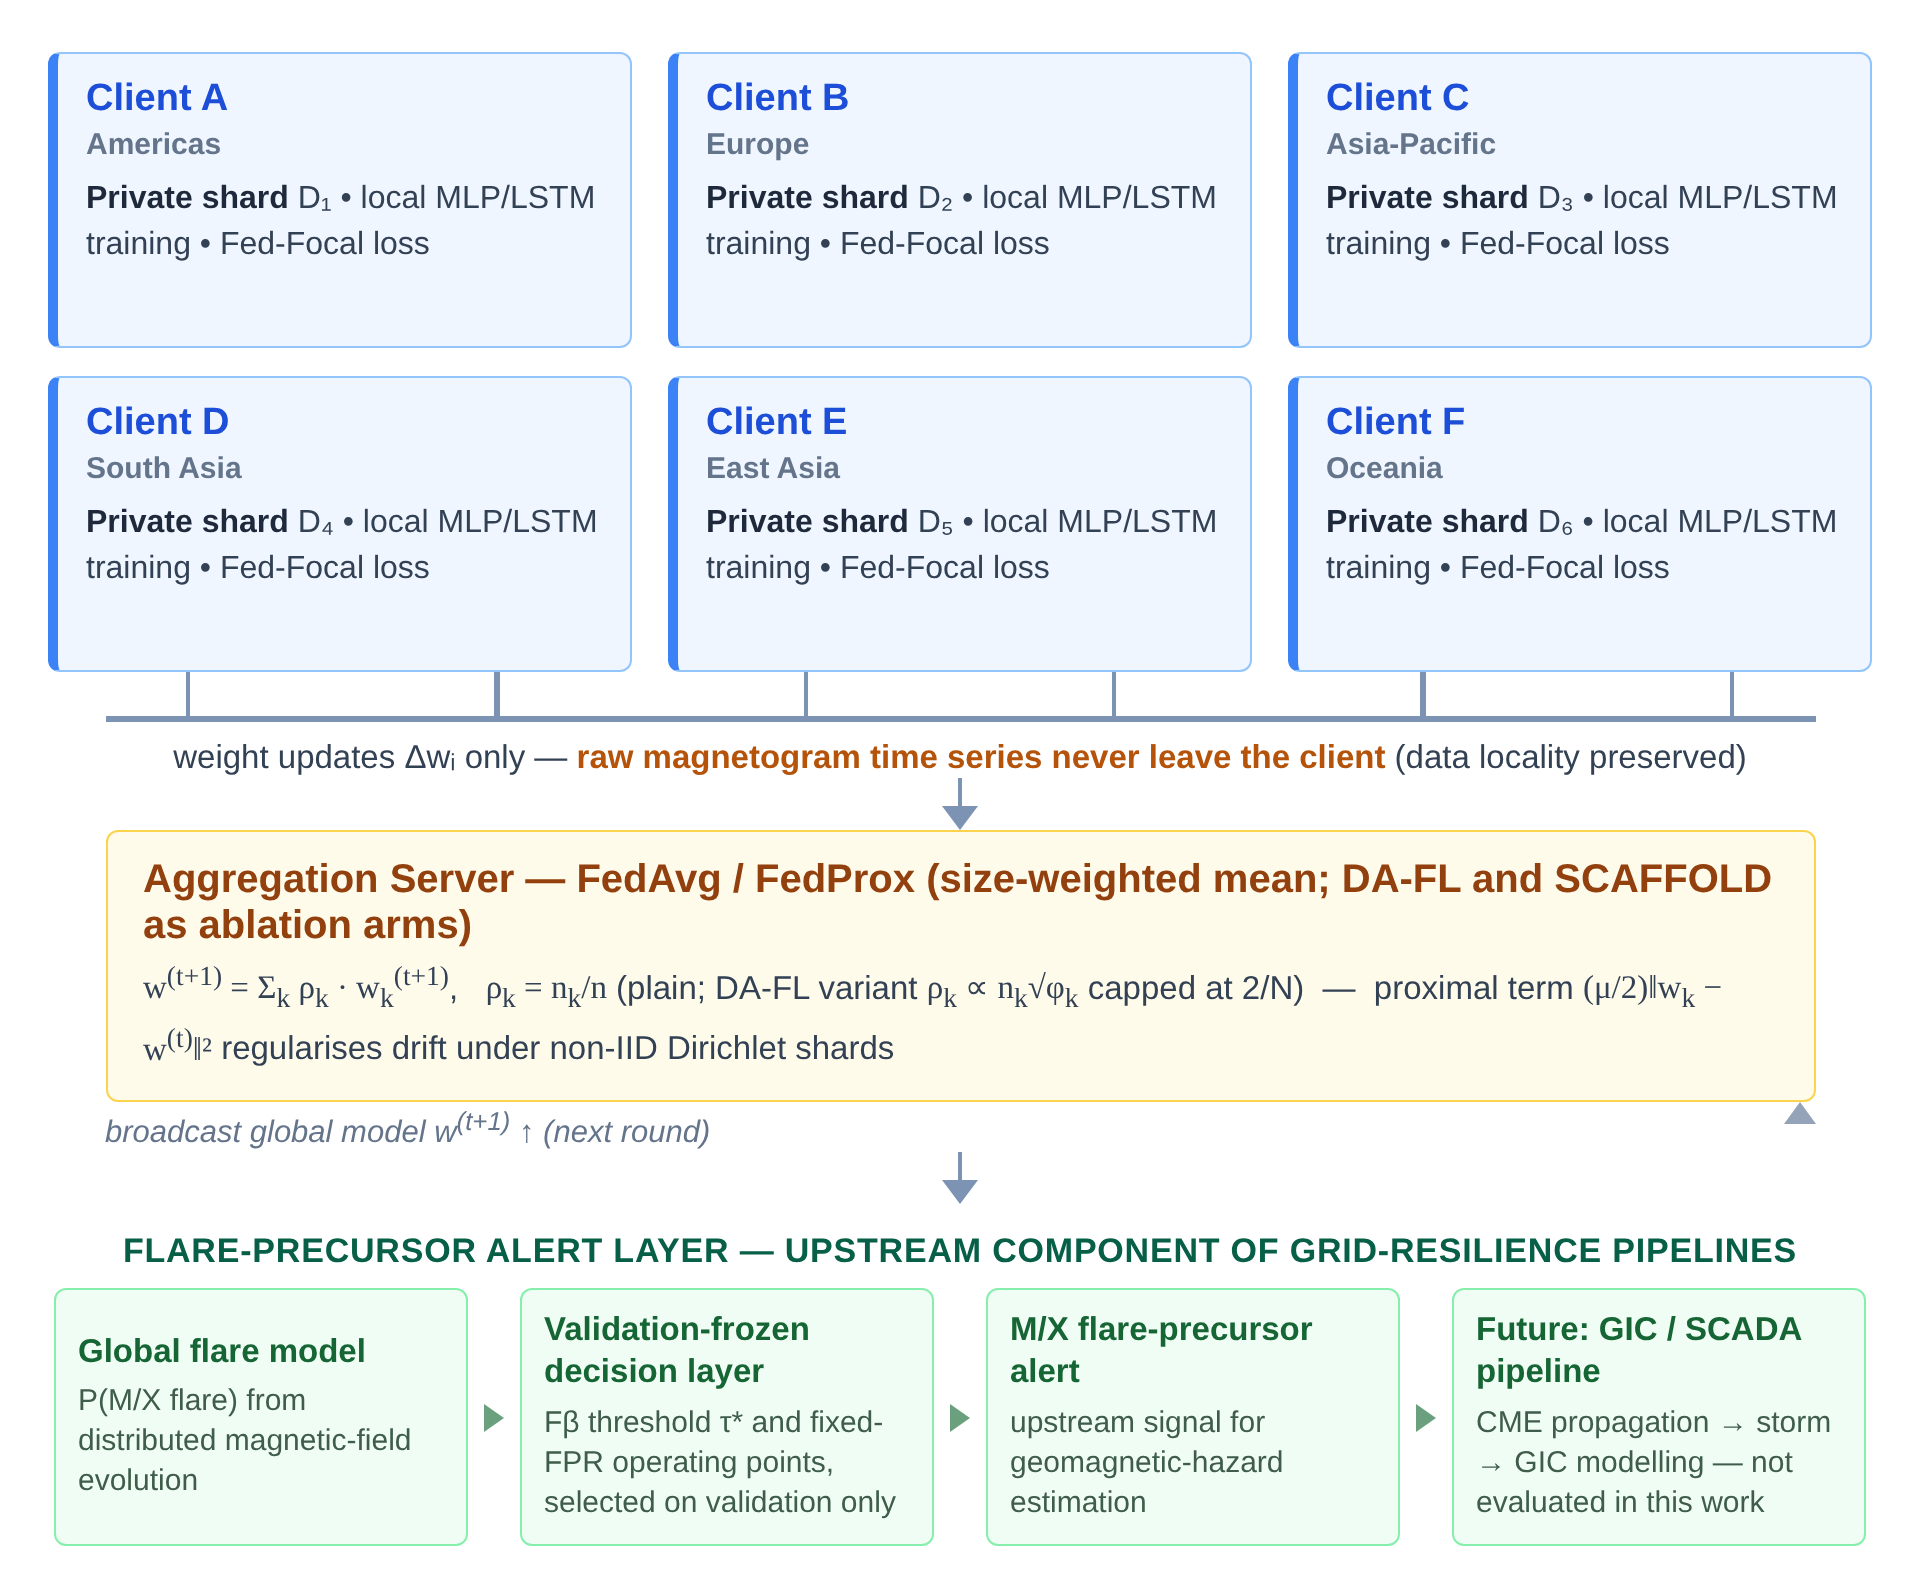
\includegraphics{figures/fig_architecture.png}
    \end{adjustbox}
    \caption{Federated benchmark-audit architecture. Six simulated
    clients (neutral labels A--F; no real institution participates)
    hold private non-IID shards of the benchmark; only model weight
    tensors $\w_k$ cross the client boundary (the figure and the
    communication-cost model describe full-weight transport; delta
    encoding is listed future compression work). The server applies
    size-weighted FedAvg/FedProx aggregation by default (the
    distribution-aware weighting $\rho_k \propto n_k\sqrt{\phi_k}$,
    capped at $2/K$, is studied as an ablation arm). The global model
    emits flare probabilities; the evaluation finds its calibration
    and frozen operating points do not survive the prevalence shift,
    so no alerting claim is made, and no downstream pipeline is
    evaluated.}
    \label{fig:arch}
\end{figure}

\subsection{Data: the SWAN-SF benchmark and its cleaned variant}

All experiments use the SWAN-SF benchmark \cite{angryk2020}
(doi:10.7910/DVN/EBCFKM), a multivariate time-series dataset of
active-region observation windows drawn from SDO/HMI vector
magnetograms, with 24 physically motivated parameters per timestep
sampled over 60-minute sliding windows and labels indicating the
occurrence of $\geq$M-class flares within the prediction horizon. The
24 parameters summarise magnetic-field complexity and include, among
others: total unsigned current helicity (TOTUSJH), total photospheric
magnetic free energy (TOTPOT), total unsigned vertical current
(TOTUSJZ), total unsigned flux (USFLUX), the sum of absolute
net-current-per-polarity (SAVNCPP), absolute net current helicity
(ABSNJZH), mean shear angle and the fraction of high-shear area
(MEANSHR, SHRGT45), the Schrijver flux-emergence proxy (R-value), and
the three components of the total Lorentz force (TOTFX, TOTFY, TOTFZ)
\cite{schrijver2007,bobra2015}.

We ingest the benchmark through its community-maintained cleaned
variant\footnote{Cleaned SWAN-SF Dataset,
\url{https://github.com/samresume/Cleaned-SWANSF-Dataset}, which
applies per-partition preprocessing: random undersampling with Tomek
links and TimeGAN-based synthetic augmentation for the training
partitions \cite{yoon2019}, LSBZM normalisation, and FPC-KNN
imputation.}, combining all five data partitions. The training
partitions are class-balanced by this preprocessing (pooled positive
rate $\bar{p} \approx 0.489$), while the untouched test partitions
retain the natural, severely imbalanced prevalence of approximately
$1.9\%$ flare windows across roughly $3.3\times10^{5}$ held-out
samples. This train--test contrast is not an artefact we introduce; it
is inherited from the benchmark's design philosophy, and it has a
consequence that shapes the entire evaluation: models trained at
$\sim$49\% prior must detect events at a $\sim$2\% prior, so absolute
probability calibration degrades and decision thresholds must be
re-optimised post hoc (Section~\ref{sec:thresholding}).

The raw-benchmark experiments of Sections~\ref{sec:res-leakfree}
and~\ref{sec:res-raw} additionally ingest the unprocessed SWAN-SF
partitions directly. The raw substrate cannot be trained on as-is:
8.87\% of its values are missing, the missingness is structured
(the Lorentz-force component TOTFZ is unobserved in 98.7\% of
training windows), and the 24 parameters span eleven orders of
magnitude. We therefore reproduce the cleaned release's two
preprocessing stages in-pipeline from their published description
(ApJS, 10.3847/1538-4365/ad7c4a) rather than inheriting their
output: a fast Pearson-correlation-based k-NN imputation (within-window
linear interpolation for partial gaps; inverse-distance-weighted
transfer of the $k{=}5$ nearest training windows' series, searched in
the space of the five most-correlated observable features, for
fully-missing series), and the LSBZM normalisation chain (robust
quantile clip, positivity shift, a log/sqrt/Box--Cox stabiliser
dispatched per feature by fitted $\lambda$, z-score, min--max), with
every parameter fitted on the training pool only and a per-feature
power-of-two pre-scaling for numerical safety. The reproduction is
verified against the released export on the audit-matched windows
(observed-position rank agreement in
Section~\ref{sec:res-raw}); where the two pipelines differ
substantively (the release re-imputes the R-value zero mass as if
missing; we preserve zeros as physical ``no flux emergence''
values), we preserve the raw semantics. The construction, the
runner, and the verification are committed as
\texttt{experiments/raw\_substrate.py},
\texttt{experiments/run\_raw\_substrate.py}, and
\texttt{experiments/run\_event\_level\_raw.py}.

\subsection{Client-side feature representation}

The framework supports two representations of the same 60-timestep
observation windows. In the MLP path used for the reported run, each
three-dimensional window $X \in \R^{60\times24}$ is reduced to a
144-dimensional statistical vector
\begin{equation}\label{eq:stats}
    \tilde{x} \;=\;
    \big[\,\mu,\;\sigma,\;\max,\;\min,\;\delta,\;s\,\big]
    \;\in\; \R^{144},
\end{equation}
where each block is applied per base feature: $\mu$ and $\sigma$ are
the temporal mean and standard deviation, $\max$ and $\min$ the window
extrema, $\delta = X_{T} - X_{1}$ the net trend, and $s$ the
least-squares slope against normalised time. This six-statistic
extraction preserves substantially more temporal information than a
temporal mean (peaks, volatility, and rate of change are precisely the
flare-relevant quantities) while remaining compatible with
weight-averaged federation and with the centralised baselines. In the
LSTM path, the raw $\R^{60\times24}$ tensor is consumed directly by a
recurrent model; this path was executed federated on the raw
substrate for all four arms plus the pooled comparator
(Section~\ref{sec:res-lstm}), with its cleaned-fold pairing remaining
future work (Section~\ref{sec:limitations}).

\subsection{Non-IID partitioning into simulated clients}

\begin{figure}[t]
    \centering
    \begin{adjustbox}{max width=0.94\textwidth, max height=0.36\textheight}
        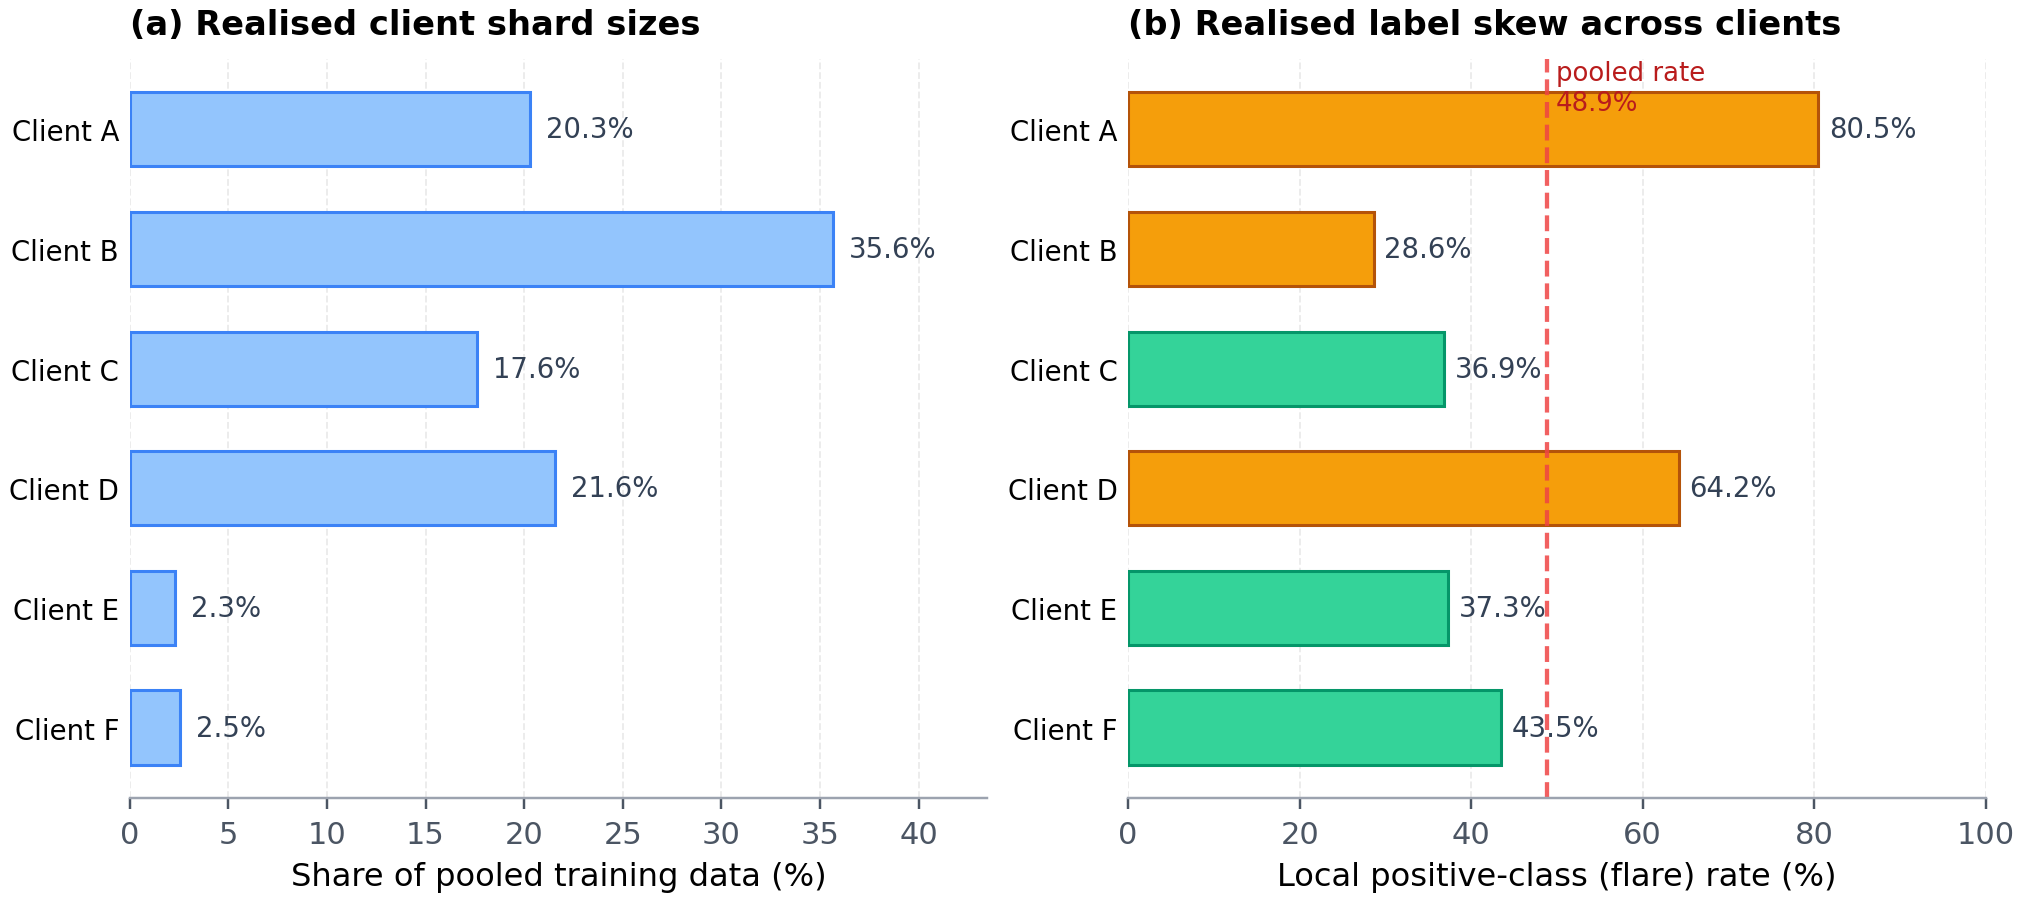
\includegraphics{figures/fig_partition.png}
    \end{adjustbox}
    \caption{Non-IID partitioning of the pooled, class-balanced
    training data into six simulated clients by label-aware Dirichlet
    sampling (concentration $\alpha = 1.0$, RNG seed 42,
    Section~\ref{sec:method}); proportions are read directly from the
    frozen run's cached client assignment. (a)~Realised relative shard
    sizes. (b)~Realised local flare rates against the pooled rate of
    48.9\%: label skew spans 28.6\%--80.5\%, emulating the label
    heterogeneity a federation would face if the shards sampled very
    different active-region populations (no real institution or
    region participates).}
    \label{fig:partition}
\end{figure}

To emulate label heterogeneity, the pooled training set is
partitioned by label-aware Dirichlet sampling: for each class $c$, a
proportion vector is drawn from
$\mathrm{Dirichlet}(\alpha,\dots,\alpha) \in \R^{K}$ and each client
receives the corresponding fraction of that class. The concentration
$\alpha$ controls heterogeneity strength---small $\alpha$ produces
near-exclusive class ownership; large $\alpha$ approaches IID.
Figure~\ref{fig:partition} shows the deterministic realisation
used by every experiment in this paper ($\alpha=1.0$, seed 42) on the
class-balanced pool: realised local flare rates span 28.6\% to
80.5\% and shard sizes range from 2.3\% to 35.6\% of the pool. This
is a deliberately hostile federation: some clients are flare-rich and
tiny, others flare-poor and large, mirroring the real asymmetry a
cross-silo federation faces when some participants' archives dominate
the pooled corpus and others sample much smaller populations. The
concentration $\alpha=1.0$
itself is the outcome of a documented tuning process
(Appendix~\ref{sec:appendix}): early experiments at $\alpha \le 0.5$
produced pathological partitions (0.3\%--99.8\% local flare rates,
re-measured under the frozen seed) under
which no aggregation scheme remained stable.

\subsection{Client models}

The primary federated architecture is a four-layer multilayer
perceptron, $\mathrm{SolarMLP}: \R^{144} \to \R$, with hidden widths
$144 \to 128 \to 64 \to 32 \to 1$, batch normalisation, ReLU
activations, and dropout $0.3$ after each hidden layer; the single
output is a raw logit consumed by the sigmoid-based losses below. MLPs
are natural federation citizens because every parameter is a
numerically meaningful averageable tensor. The released framework also
implements $\mathrm{SolarLSTM}$, a (optionally bidirectional) two-layer
LSTM with hidden size 128, Xavier/orthogonal initialisation, and a
forget-gate bias of one for long-horizon memory, followed by a
two-layer classification head \cite{hochreiter1997,hassani2025}. Local
training uses AdamW \cite{loshchilov2019} with cosine-annealing warm
restarts and gradient-norm clipping at $5.0$. We deliberately keep
XGBoost out of the federation loop: gradient-boosted tree ensembles
store discrete structure that cannot be meaningfully averaged, so the
centralised XGBoost serves as the pooled upper bound rather than a
federated participant.

\subsection{Federation algorithms and aggregation}

Three cross-silo algorithms are implemented. \textbf{FedAvg}
\cite{mcmahan2017}: each round, every client initialises from the
broadcast global model, performs $E=10$ local epochs, and the server
averages the returned weights. \textbf{FedProx} \cite{li2020}: identical
to FedAvg except each client's local objective is regularised by the
proximal term of Eq.~\eqref{eq:fedprox} with
$\mu = 0.01$, penalising drift from the global model---the mechanism
we hypothesise is decisive under the label skew of
Figure~\ref{fig:partition}. \textbf{SCAFFOLD} \cite{karimireddy2020}:
variance reduction via client and server control variates; it is
implemented with the SGD-based update required for exactness of the
control-variate correction (AdamW's adaptive steps would invalidate
the correction terms). Five implementation details depart from the
reference algorithm and are disclosed for exactness: (i)\ the
control-variate correction is damped, rescaled to 10\% of each
parameter's gradient norm (the undamped correction destabilised
training on this benchmark's loss scale); (ii)\ gradients are clipped
to max-norm 1.0; (iii)\ the shipped optimiser is SGD with momentum
$0.9$ at a learning rate of $2.5\times10^{-4}$ --- half the global
rate --- a departure of a milder class, since momentum biases the
average-gradient estimate that the control-variate update divides by
(disclosed at v4.5); (iv)\ the client control-variate update is
\emph{sign-inverted} relative to Eq.~11 of the reference algorithm:
the repository computes
$c_i^{+} = c_i - c + (y_i^{+} - y_i)/(\eta K)$ --- the negative of
the client's average local gradient --- where Karimireddy et
al.\ specify $c_i^{+} = c_i - c + (y_i - y_i^{+})/(\eta K)$; a
scalar one-client simulation of the code path confirms the inversion
exactly (the update evaluates to $-1.0000$ times the average local
gradient), and the wrongly-signed variate estimates push the
correction term $c - c_i$ the wrong way over rounds --- the damping
of item~(i) and the variate clamping bound the damage, which is why
the arm still trains (found by Dossier R-FS9-R6, disclosed at
v4.6); and (v)\ the arm is trained \emph{cold}: on every path that
produced a published operating point --- the raw-substrate MLP and
LSTM arms --- the model starts from a fresh random initialisation at
half the global learning rate, not from a converged FedAvg model
(the FedAvg-initialised warm start claimed at v3.9--v4.5 exists only
on the cleaned-fold path, where the arm is never executed; the v4.6
correction follows the call sites and the queue log, whose
validation F1 is pinned at zero through round thirty --- the
cold-start signature). A cold start at half the global rate is a
\emph{harder} protocol than the FedAvg-initialised refinement
previously claimed, so the arm's published trajectory should be read
as a from-scratch run. One further arm-level asymmetry is disclosed
at v4.5: the published SCAFFOLD operating points were trained before
the imbalance factor's global-prevalence fix (founding-audit finding
B13) was extended to the SCAFFOLD local path, so that arm's focal
weight used the hardcoded cleaned-substrate prevalence $0.4887$ as
$\bar{p}$ rather than the computed global rate the FedAvg and
FedProx arms use; on the roughly two-percent-positive raw substrate
the imbalance factor saturates at its clamp either way, which bounds
the effect. The call site is aligned at v4.5, so all three federated
arms share one loss definition in the released code, and the same
alignment is extended at v4.6 to the centralised comparators (the
pooled MLP, the budget-matched re-run, and the pooled LSTM), whose
published operating points likewise predate the plumbing and trained
under the same hardcoded-prevalence fallback --- an asymmetry of
exactly the bounded class disclosed above for the SCAFFOLD arm,
disclosed here for the central side as well (Dossier R-FS9-R6,
R8-5). Because every
published SCAFFOLD operating point was produced by this
implementation, the arm's comparisons against its siblings measure
\emph{this implementation}, not the reference algorithm: the
raw-substrate cells of Sections~\ref{sec:res-raw}
and~\ref{sec:res-lstm} --- the MLP instance's hardest-failure mode
and the sequence instance's highest event-level detection --- are
implementation-case evidence for a sign-inverted, cold-start,
damped SCAFFOLD, and a sign-corrected, warm-started vanilla
replication under the frozen protocol is queued owner-GPU future
work whose outcome may differ. The arm was held out of the
cleaned-substrate headline configuration for stability reasons and
is not run on the cleaned fold, but it is executed on the raw
substrate for both encoders, where its MLP instance is the hardest
failure and its sequence instance completes the four-arm federation
matrix (Sections~\ref{sec:res-raw} and~\ref{sec:res-lstm}).

Aggregation is \emph{plain size-weighted averaging} in the frozen
headline configuration ($\rho_k = n_k/n$, the vanilla FedAvg
choice); distribution-aware weighting (DA-FL), in which the server
weights client $k$'s update by
\begin{equation}\label{eq:dafl}
    \rho_k \;\propto\; n_k \sqrt{\phi_k},
    \qquad
    \phi_k = \frac{p_k}{\bar{p}},
    \qquad
    \rho_k \le \frac{2}{K},
\end{equation}
with $p_k$ the client's local positive rate and $\bar{p}$ the pooled
rate known to the server, is implemented as an \emph{ablation arm}
(Section~\ref{sec:res-ablation}). The square-root damping and the
$2/K$ cap prevent a flare-rich client from dominating the global
model while still up-weighting the clients most likely to contain
decision-relevant minority samples. Class-rate metadata is
deliberately much coarser than raw data and is treated as shareable
under the data-locality constraint.

\subsection{Fed-Focal loss and local rebalancing}

Each client trains with a server-aware focal loss in the Fed-Focal
family \cite{sarkar2020},
\begin{equation}\label{eq:focal}
    \ell_{\mathrm{fedfocal}}
    \;=\; -\,\alpha_t\,\bigl(1 - p_t\bigr)^{\gamma}
    \log\bigl(p_t\bigr),
    \qquad \gamma = 2.0,
\end{equation}
where $p_t$ is the model's probability of the correct class and
$\alpha_t$ interpolates between $\alpha$ and $1-\alpha$ by label. The
positive-class weight $\alpha$ is computed per client as the base value
$0.25$ \cite{lin2017} scaled by a square-root-damped imbalance factor
$\min\!\big(\sqrt{\bar{p}/p_k},\,1.5\big)$ --- with the client rate
floored at $\max(p_k, 0.01)$ so a flare-free client cannot divide by
zero --- and a mild round-progress factor in $[0.9,\,1.1]$
(linear in round progress; the $[0.7,\,1.3]$ range of an earlier
revision inflated $\alpha$ past its clamp), then clamped to
$(0.05, 0.25)$. Both constants are v4.6 disclosures completing the
loss definition (Dossier R-FS9-R6 R8-12). This clamping is a hard-won
design decision: unclamped adaptive weighting (earlier versions allowed
$\alpha$ up to $0.95$) systematically inflated positive-class weight on
flare-poor clients, producing degenerate always-flare classifiers with
recall $\approx 1.0$ and precision $\approx 0.03$
(Appendix~\ref{sec:appendix}). NaN-safe clamping of $p_t$ and of the
loss itself guards the pipeline against logit explosions in early
rounds. The framework additionally supports per-client SMOTE
oversampling \cite{chawla2002} and mixup \cite{zhang2018}; both are
\emph{disabled} in the frozen configuration because the cleaned
benchmark's training partitions arrive pre-balanced (48.9\% positive),
which renders SMOTE inert---the configured oversampling ratio produces
zero synthetic samples. The balancing question is therefore
inapplicable to this benchmark variant, and we report it as a null
result rather than a contribution (Section~\ref{sec:res-ablation});
on the raw substrate, where natural prevalence gives it work to do,
the per-client SMOTE ablation has since been executed and is
likewise a clean negative (Section~\ref{sec:res-lstmrep}).

\subsection{Threshold protocol for safety-critical recall}
\label{sec:thresholding}

Because federated training operates on rebalanced local data while
deployment operates at the natural $1.9\%$ prior, the emitted
probabilities are deliberately miscalibrated, and a fixed $0.5$
threshold is meaningless. The frozen protocol therefore performs all
selection on validation data, in two stages. First, the decision
threshold is selected by sweeping $\tau$ over $[0.05, 0.95]$ in steps
of $0.005$ and choosing, per model, the $\tau^\ast$ that maximises
$\Fbeta$ with $\beta=2$ (Eq.~\eqref{eq:fbeta}) on the validation set;
$\tau^\ast$ is then frozen and applied to the test set exactly once.
All reported precision, recall, F1, and accuracy figures are taken at
each model's frozen threshold. Second---because balanced-prevalence
validation turns out not to support threshold transfer at all
(Section~\ref{sec:res-calib})---the framework additionally freezes
\emph{fixed-FPR operating points}: for each target false-positive
budget $f \in \{0.5\%, 1\%, 2\%, 5\%\}$, the threshold is set to the
$(1-f)$-quantile of \emph{validation negative scores}, a quantity that
uses no test information whatsoever; the realised test behaviour at
each frozen threshold (achieved FPR, recall, precision, alert rate) is
reported in the same single test pass. The negative-quantile rule is
numerically validated in the released test suite, and the
raw-substrate retraining of Section~\ref{sec:res-raw} supplies the
natural-prevalence validation split that is the ideal substrate for
this protocol.
ROC-AUC and PR-AUC, being threshold-free, are reported independently.

\subsection{Threat model and security posture}
\label{sec:threatmodel}

The verified property of this framework is data locality (raw data
never leaves the client), not end-to-end security. To make that scope
auditable, Table~\ref{tab:threat} states the threat model explicitly:
which adversaries are considered, which defences the released code
provides, and which are documented but unevaluated.

\begin{table}[t]
\centering
\caption{Threat model of the released framework. ``Mitigated in code''
means implemented and covered by the integrity test suite;
``documented'' means design guidance exists but no quantitative
evaluation has been performed on this benchmark.}
\label{tab:threat}
\small
\begin{tabularx}{\textwidth}{@{}>{\raggedright\arraybackslash}X >{\raggedright\arraybackslash}X >{\raggedright\arraybackslash}X@{}}
\toprule
\textbf{Adversary / attack} & \textbf{Defence} & \textbf{Status} \\
\midrule
Honest-but-curious aggregation server (observes all weight
updates) & Secure-aggregation module (Bonawitz-style masks;
tests verify arithmetic round-trip cancellation only --- the sketch
uses deterministic, publicly reproducible mask keys, so it confers
no cryptographic privacy as committed) & Implemented as a numerical
sketch; not wired into the training loop; accuracy overhead not
measured \\
\addlinespace[2pt]
Gradient inversion / reconstruction from the transcript
$\mathcal{T}$ \cite{zhu2019} & Secure aggregation (masks updates);
differential-privacy hooks & Documented; not evaluated \\
\addlinespace[2pt]
Membership inference against a specific client's training data &
Differential-privacy hooks (noise on client updates) & Documented;
not evaluated \\
\addlinespace[2pt]
Malicious client: model poisoning / backdoor insertion & None at
present; Byzantine-robust aggregation is a design note & Not
addressed \\
\addlinespace[2pt]
Client impersonation / spoofed updates & Transport security (TLS)
and client authentication are deployment infrastructure outside the
learning loop & Documented (deployment guidance) \\
\addlinespace[2pt]
Network interception of updates & TLS in transit & Documented
(deployment guidance) \\
\bottomrule
\end{tabularx}
\end{table}

For the benchmark study reported here---six simulated clients, public
data, no real adversaries---none of these defences is enabled, so the
reported accuracy numbers are those of the undefended pipeline. Any
cross-agency deployment would need to re-measure accuracy under secure
aggregation and differential privacy before the numbers in
Section~\ref{sec:results} could be quoted as expected operational
performance (Section~\ref{sec:limitations}).

\subsection{Interpretability layer}

To audit what the models learn, SHAP values \cite{lundberg2017} are
computed for the centralised XGBoost reference over a 500-sample test
subset with the TreeExplainer and for the federated model with DeepSHAP
(100-sample background), yielding mean absolute SHAP attributions per
feature. The statistical representation of Eq.~\eqref{eq:stats}
carries a 144-entry name contract---each feature is named
\texttt{<statistic>\_<parameter>} (e.g.\ \texttt{mean\_TOTUSJH},
\texttt{max\_R\_VALUE}), with the statistic blocks ordered $\mu$
(0--23), $\sigma$ (24--47), $\max$ (48--71), $\min$ (72--95), $\delta$
(96--119), $s$ (120--143) over the 24 base parameters---and the
improved pipeline preserves these names end-to-end, so the SHAP layer
reports physically meaningful attributions directly (the v2.x pipeline
lost the mapping and required an analytical decoding pass;
Appendix~\ref{sec:appendix}). Section~\ref{sec:results} presents the
raw ranking, its statistic-level structure, and the physical grouping
used for cross-model comparison.
